\documentclass[pdftex,12pt,a4paper]{report}

\usepackage[pdftex]{graphicx}
%\usepackage[ansinew]{inputenc}
\usepackage{geometry}
\usepackage{bbold}
\usepackage[T1]{fontenc}
\usepackage[utf8]{inputenc}
\usepackage[english]{babel}
\usepackage{url}
\usepackage{subfigure}
\usepackage{hyperref}
\usepackage[section]{placeins}
\usepackage{listings}
\usepackage{wrapfig}

\usepackage[table,xcdraw]{xcolor}
\geometry{a4paper,left=2.5cm,right=2.5cm, top=2.5cm, bottom=3cm}
\newcommand{\HRule}{\rule{\linewidth}{0.5mm}}

%\usepackage{titlesec}
%\titleformat{\chapter}[display]
%  {\normalfont\bfseries}{}{0pt}{\Huge}

\usepackage[Sonny]{fncychap}
\makeatletter
\ChTitleVar{\Large\rm\centering} % sets the style for title
\ChNameLowerCase
\renewcommand{\DOCH}{}
\makeatother

\begin{document}
\begin{titlepage}


%%LR
\sffamily

\begin{center}


% Oberer Teil der Titelseite:

\includegraphics[width=0.3\textwidth]{bilder/logo2.jpg}
\hfill

\includegraphics[width=0.4\textwidth]{bilder/logo1.jpg}  
\\[5cm]

{\Large Bioinformatics Program}\\[0.5cm]
{\Large Technical University of Munich}\\[0.5cm]
{\Large Ludwig-Maximilians-Universit\"at M\"unchen}\\[2cm]
{\Large Master's Thesis in Bioinformatics}\\[1.5cm]

% Title
\HRule \\[0.4cm]
{ \huge \bfseries Patient-specific Dysregulation Analysis Based on Gene Regulatory Networks in Cancer}\\[0.4cm]

\HRule \\[1.5cm]

{\Large Sebastian Dötsch}\\[2.5cm]

\vfill
\end{center}
\end{titlepage}
\pagestyle{empty}

%%LR comprehensive title
\begin{titlepage}
{\sffamily


\begin{center}

\includegraphics[width=0.3\textwidth]{bilder/logo2.jpg}
\hfill

\includegraphics[width=0.4\textwidth]{bilder/logo1.jpg}  
\\[3cm]  

{\Large Bioinformatics Program}\\[0.5cm]
{\Large Technical University of Munich}\\[0.5cm]
{\Large Ludwig-Maximilians-Universit\"at M\"unchen}\\[2cm]
{\Large Master's Thesis in Bioinformatics}\\[2cm]
{\textbf{\LARGE Patient-specific Dysregulation Analysis Based on Gene Regulatory Networks in Cancer}}\\[2cm]
{\textbf{\LARGE Patientenspezifische Dysregulationsanalyse bei Krebs basierend auf genregulatorischen Netzwerken}}\\[3cm]

\end{center}
\begin{center}\Large
  \begin{tabular}{ll}
    Author:& Sebastian Dötsch\\
    Supervisor: &  Dr. Markus List Chair of Experimental \\
    & Bioinformatics,\\
    & TUM School of Life Sciences Technical University\\
    & of Munich \\
    & Dr. Josch Pauling LipiTUM, Chair of Experimental \\
    & Bioinformatics, \\
    & TUM School of Life Sciences Technical University\\
    & of Munich \\
    Advisor:        &  Alexander Dietrich, Technical University of Munich\\
    Submitted:     &  15.10.2023
  \end{tabular}
\end{center}

}% end title page

\end{titlepage}

\newpage
\phantom{oben}
\vfill
\begin{center}
\large\textbf{Declaration of Originality}\normalsize\\
\vspace{0.5cm}
I confirm that this master's thesis is my own work and I have documented all sources and material used.\\
\vspace{1.5cm}
\begin{tabular}{lp{2em}l}
 \hspace{3cm}   && \hspace{3cm} \\\cline{1-1}\cline{3-3}
 Place, Date     && Signature
\end{tabular}
\end{center}
\vfill

\tableofcontents

\chapter*{Abstract}
Gene expression is highly regulated by non-coding regulatory elements of DNA, which can be influenced by diseases including cancer. These can be located close or distant to their respective gene and form complex regulatory systems. DNA methlyation represents one of the epigenetic modifications that regulates gene expression through inhibition or repression. Alteration of this regulation in cancer patients leads to oncogenesis and uncontrolled cell growth. The presented network based approach aims to reveal patient-specific gene regulatory network dysregulations in breast cancer tissues.

For this purpose, the EpiRegioDB database, which contains epigenetic data on regulatory elements and their genes, was used as the basis for creating gene regulatory networks. A web app was designed to visualise and explore the nodes, edges and relationships of the gene regulatory networks.  A publicly available breast cancer dataset was used to find dysregulations within the gene regulatory network using the DysRegNet tool. The investigation of the dysregulations and their corresponding transcription factor binding sites with the enrichment tool LOLA yielded promising results. Dysregulated transcription factor binding sites were found for the proteins EZH2, SUZ12, H3K26me3 and CtBP2, which are already associated in the literature with altered regulation in breast cancer. The results show that the approach can identify known dysregulated regulatory elements. This raises the possibility of identifying new dysregulations and their regulatory elements in disease tissues. New insights can pave the way for a more profound understanding of epigenetic diseases and open up new therapeutic approaches.\\\\
Code and produced data is available at https://github.com/doetschs/REMnet.
 
\chapter{Introduction}

\section{Epigenetics}
The word epigenetics is a compound of the words epi - Greek for above - and genetics, which describes changes in gene expression that are "above"/"on top" and independent of changes in the primary DNA sequence\cite{epigenetics2}.
As a field at the intersection of genetics and molecular biology, epigenetics gives insights into heritable an stable long-term alterations in gene regulation. It involves dynamic changes in DNA, chromatin, and non-coding RNAs. Histone tail modifications, including acetylation and DNA methylation are examples of mechanisms that cause these alterations. They control chromatin structure and influence gene accessibility\cite{epigenetics_histone}. Non-coding RNAs such as microRNAs on the other hand fine-tune gene expression post-transcriptionally. Epigenetics thus offers insights into development, disease, and therapeutic opportunities\cite{epigenetics_nonRNA}. The dynamic interplay between genetic and epigenetic mechanisms opens new approaches for our understanding of biological complexity and is therefore investigated.
\subsection{DNA Methylation}
DNA methylation, an important epigenetic modification, involves the addition of methyl groups to cytosine or adenine bases in DNA molecules. It typically occurs on the first mentioned by addition of the methyl group to the carbon-5 atom of cytosine. This reaction is catalyzed by the three DNA methyltranferases DNMT3A, DNMT3B and DNMT1. DNMT3A and DNMT3B are essential for de novo methylation, for example during embryogenesis and germ cell development \cite{methylation_dnmtsAB}. DNMT1 on the other hand is responsible for maintaining methylation patterns and does this by catalyzing the addition of methyl groups to cytosine nucleotides \cite{methylation_dnmts1}. Therefore this chemical alteration is involved in cellular development and maintenance of genome integrity. It regulates gene expression by inhibiting the binding of transcription factors (TFs) to DNA or recruiting repressor genes \cite{gene_regulation}. It additionally silences a large number of parasitic transposable, retroviral, repeat elements, which the mammalian genome gathered over time \cite{MethRole}.

DNA methylation occurs very frequently at CpG sites (CpGs), 70\% to 80\% of CpG cytosines are methylated in mammals\cite{methylation_cpg}.
CpGs are regions in the DNA where a cytosine nucleotide is followed by a guanine nucleotide, if they occur with a atypically high frequency in a sequence it is called a CpG island\cite{cpgislandguide}.
These sites hold a central role in gene expression regulation, acting as epigenetic switches when located in promoter regions of genes\cite{cpgisland}. 
Beta values, a critical metric in DNA methylation studies, quantify the degree of DNA methylation at CpG sites. By taking the methylated (\emph{M}>0) and unmethylated (\emph{U}>0) signal intensities, measured by the Illumina 450k array for instance, the beta value \emph{b}=\emph{M}/(\emph{M}+\emph{U}+\emph{a}) is calculated. To stabilize beta values when \emph{M} and \emph{U} are small, the offset $\emph{a}\geq0$ usually equal to 100 is added to \emph{M}+\emph{U}. Ranging from 0, completely unmethylated, to 1, completely methylated, beta values provide a quantitative measure of DNA methylation levels. They are instrumental in understanding epigenetic modifications associated with diverse biological processes, from normal development to diseases like cancer\cite{mvalues}.

Analyzing beta values enables researchers to identify differentially methylated CpG sites, crucial for biomarker discovery and understanding disease mechanisms. This quantitative approach to epigenetics grants insights into the dynamic nature of DNA methylation, understanding their role in health and disease.
\subsection{Regulatory Elements}
Gene regulation is a finely-tuned process in which several molecular components play crucial roles. Cis and trans gene regulatory elements (REMs) are pivotal components of this process.
Cis elements, non-coding DNA regions, are located proximal to specific genes and encompass promoters and enhancers. Promoters initiate gene transcription, while enhancers enhance gene expression. Cis elements often act as transcription factor binding sites (TFBs) for trans acting factors\cite{rems_enhancers}.
Trans elements are represented by TFs, regulating the expression of distant genes by precisely binding to cis elements. In most cases such complex interactions between cis regulatory elements and trans acting factors regulate gene expression. TFs are responsible for regulating the timing and location of gene transcription\cite{rems_cis_trans}. They serve as molecular switches, exerting control over gene activation or repression. TFs play indispensable roles in cellular processes, including differentiation and response to external stimuli\cite{rems_enhancers}.

\section{EpiRegioDB}
The EpiRegio\cite{Epi} project includes a database and web server that aim to advance
epigenomic research by providing a centralized and accessible platform for analyzing and
exploring epigenetic data. 

EpiRegio serves as a comprehensive resource for exploring epigenetic data including gene expression, REMs and their interactions. It integrates data from Roadmap\cite{roadmap} and Blueprint\cite{blueprint} and provides a user-friendly interface for data retrieval and analyses. The project aims to enable researchers to investigate epigenetic patterns across diverse cell types, tissues, and organisms by providing data about regulatory elements, their assigned genes and their regulation as previously explained. By consolidating data from multiple experiments and studies, EpiRegio enables researchers to gain insights into the role of epigenetic modifications in gene regulation and disease processes.

The project offers various features and tools to support epigenomic research. It provides data visualization capabilities, statistical analysis tools, and a search and query function to locate specific epigenetic marks or genomic regions of interest. The web server offers several visualization options, such as genomic tracks, heatmaps, and scatter plots, to facilitate the exploration and interpretation of epigenomic data. Additionally, users can perform statistical analyses to identify differentially methylated regions and other epigenetic features.

Overall, the EpiRegio project aims to accelerate scientific discoveries and advance the understanding of epigenetic mechanisms in health and disease.


\subsection{Regulatory Elements in EpiRegioDB}
EpiRegio contains data on REMs and information about their activity in different tissues, cell types, their target gene and its expression\cite{regelements}. 

\begin{figure}[!ht]
\begin{center}
	\fbox{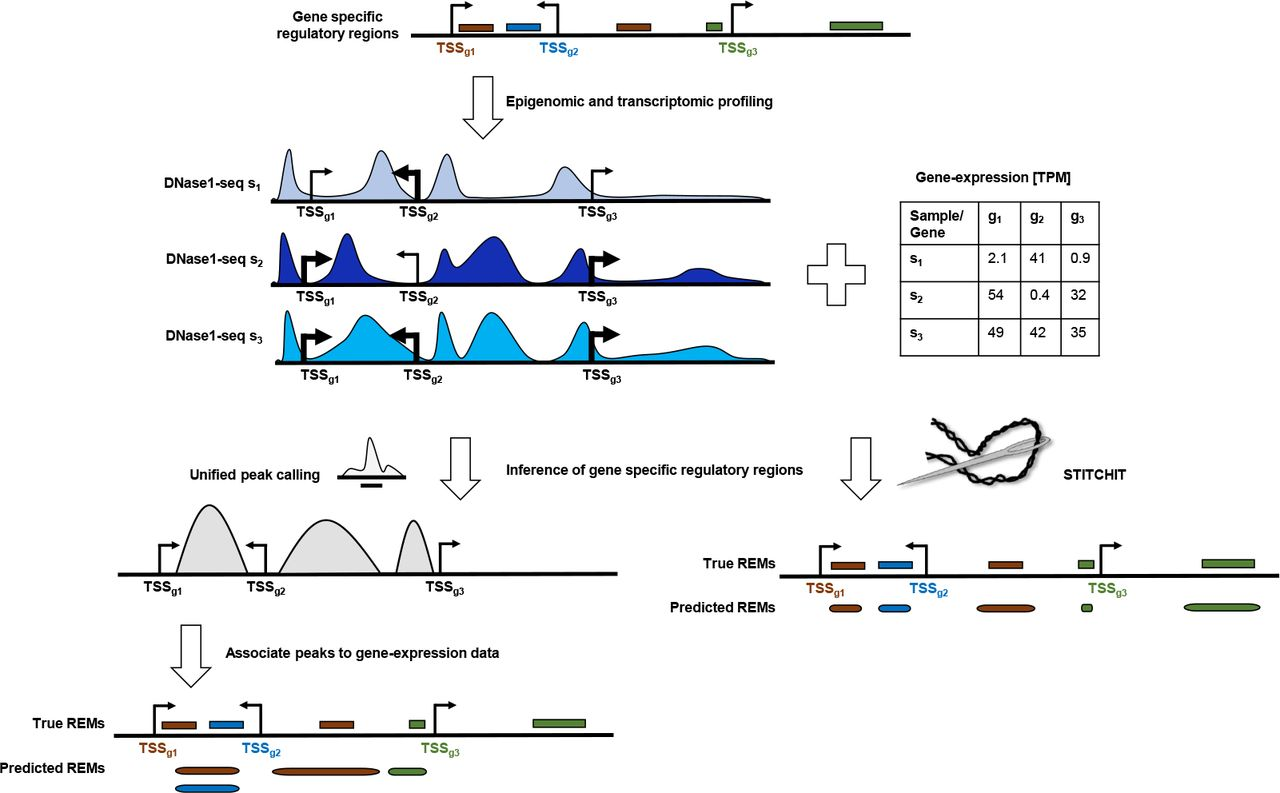
\includegraphics[scale=1.3]{figures/stitchit.jpg}}
	\caption{An Illustration of the STITCHIT method and its performance compared to peak-calling methods. Figure taken from \cite{stitchit} without modifications under the Creative Commons CC-BY license.}
	\label{stitchit}
\end{center}
\end{figure}
REMs in EpiRegio are predicted using STITCHIT\cite{stitchit}, which is a method to identify gene-specific REMs based on the analysis of epigenetic signal of diverse human cell types with respect to gene expression. STITCHIT does this by solving a classification problem in which it segments a large genomic area around the target gene (Fig. \ref{stitchit}). A linear regression using elastic-net penalty for feature selection and an Ordinary Least Squares regression to get a final regression coefficient and P-value are used. Regions exhibiting the epigenetic signal variance, which is linked to the expression of the gene, are highlighted in the resulting segmentation. Because STITCHIT is a peak-calling free approach it is able to identify REMs with high resolution and accuracy. Since genomic locations are not exclusive to REMs, REMs associated to different genes can overlap. Therefore Cluster of Regulatory EleMents (CREMs) are introduced, containing all, at least two, REMs overlapping with each other by at least one base pair without any break in between. 
In EpiRegio mentioned REMs, CREMs and their target gene are stored with multiple attributes. REMs and CREMs are stored with unique IDs, chromosome, start position and end position. Genes are stored with their Ensemble ID, also chromosome, start position, end position and their expression value in the respective cell type and sample. The linkage between CREMs and REMs and genes has the following activity values:

I) The \texttt{Model score} is a indicator on how important a REM is for the target gene expression compared to all other REMs assicated with that gene. The score is the absolute binary logarithm of the p-value of the regression coefficient for the connection between a REM and its associated gene. It is normalized with the maximal value to obtain a model score in the range [0, 1]. The larger the score, the more impact the REM has on the gene and vice versa. It is not cell type specific, thus can be used for comparison between REMs but not in between cell types.

II) The \texttt{StandDnase1Log2} score is a measurement for the accessibility of the chromatin in the REMs, indicating the activity of a REM to its target gene. It is the Deoxyribonuclease 1 (DNase1) signal for a REM retrieved from the Roadmap\cite{roadmap} and Blueprint\cite{blueprint} data sets. DNase1 is an endonuclease coded by the human DNASE1 gene, which functions by cleaving DNA in an endonucleolytic manner\cite{dnase_nih}. The signal is retrieved by the DNase 1-seq method\cite{dnase_method} and has been used as indicator for regulatory regions, which have been shown to map many types of cis regulatory elements. The DNase1 signal is log-transformed and standardized over all cell types\cite{dnase_cis}. The value inticates how active a REM is in a cell type for a sample and therefore allows the for the comparison between samples, since it is normalized for sequencing depth. 
\section{Gene Regulation}
\begin{wrapfigure}{r}{0.5\textwidth}
	\fbox{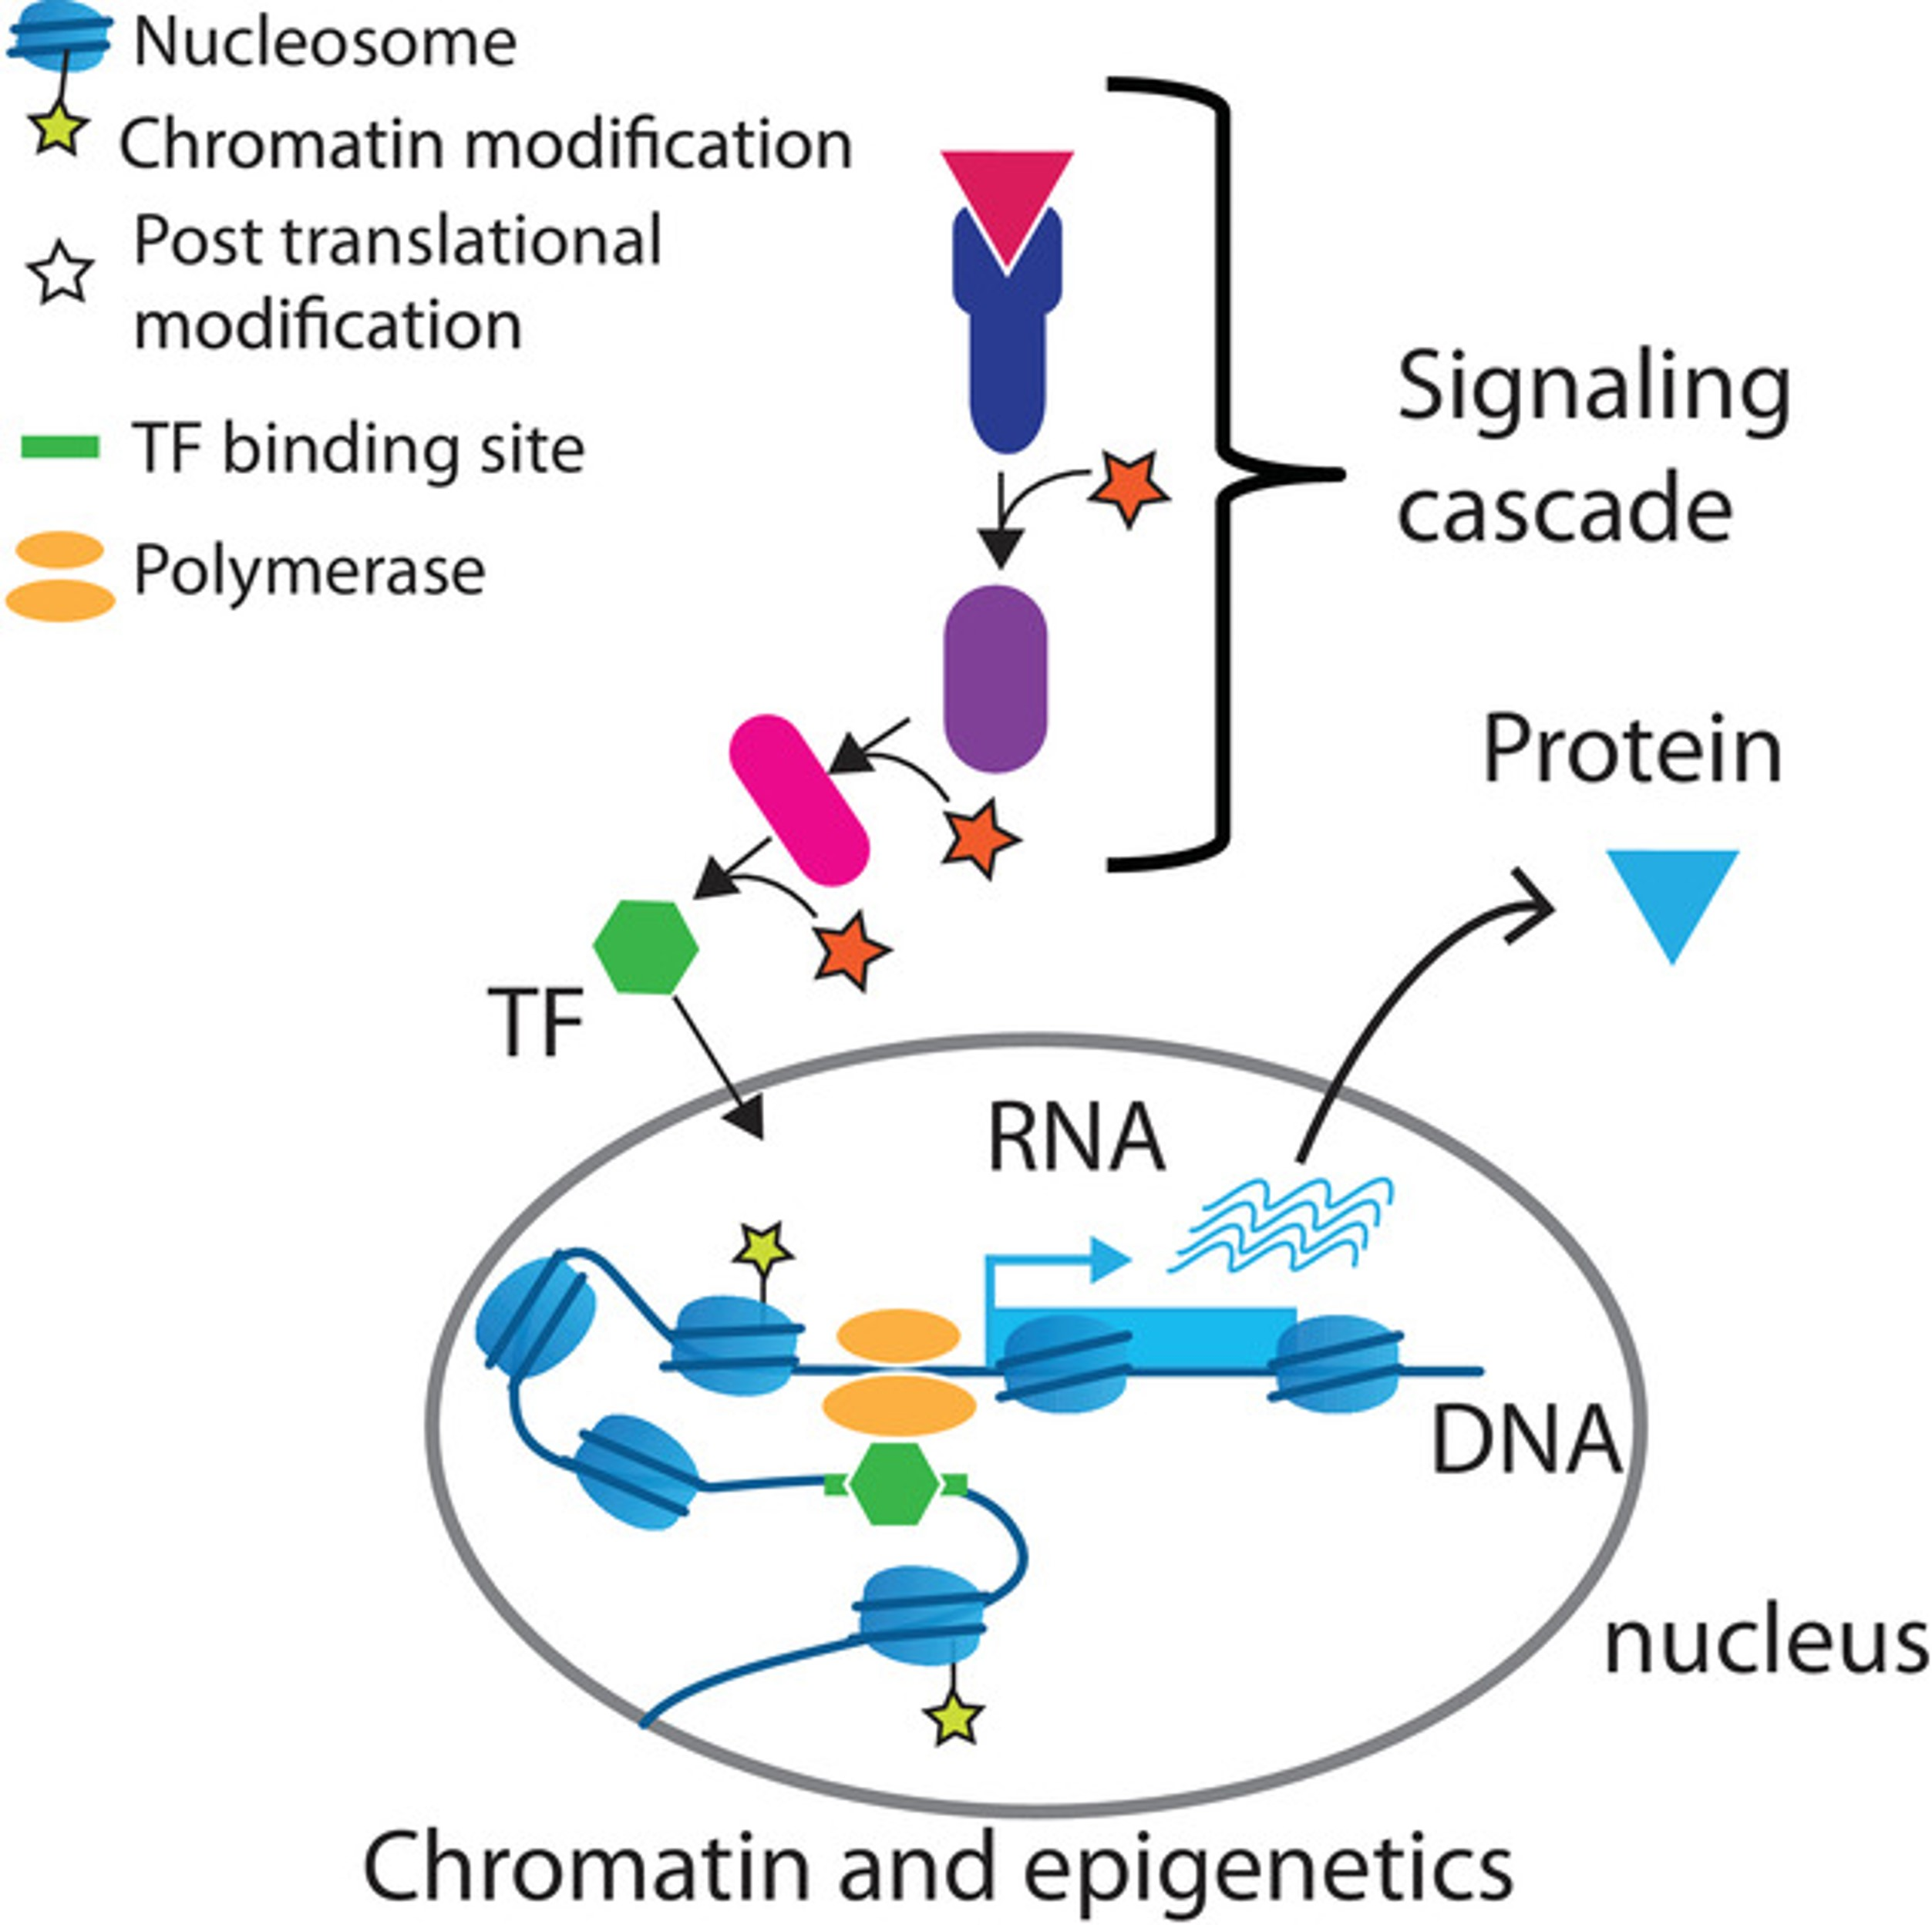
\includegraphics[scale=0.7]{figures/TF_function.jpg}}
	\caption{A simplified view of the TF activity in gene expression regulation. Figure taken from \cite{TF_fig} without modifications under the Creative Commons CC-BY license.}
	\label{TF_function}
\end{wrapfigure}
Gene regulation is a fundamental biological process necessary for the proper functioning of cells and organisms. Genes contain the instructions for the synthesis of proteins, which perform essential tasks within cells, such as providing structural support, acting as transporters or catalyzing chemical reactions. However, not all genes should be active all the time. Gene regulation ensures that genes are activated or suppressed as needed to adapt to changing conditions and maintain cellular order.
Therefore the regulation process is not static, they exhibit dynamic behaviors, responding to developmental cues and environmental stimuli\cite{GRN2}. 
This leads to a precise control over the timing and amount of the protein synthesis, which is crucial for the normal functioning of cells and the overall development of an organism.\cite{proteinfunction}.
Gene regulation relies on a complex system involving TFs, enhancers, and epigenetic modifications and often build a larger regulatory network. In this system TFs bind to specific DNA sequences in gene promoters and enhancers. By binding, they modulate the initiation and level of transcription, either activating or repressing gene expression. Activators facilitate the recruitment of RNA polymerase, essential for transcribing the gene into mRNA, while repressors inhibit this process (Fig \ref{TF_function}). These factors often operate in combinations, enabling precise and context-dependent control of gene activity. Epigenetic modifications, like DNA methylation and histone modifications, further modulate gene accessibility\cite{TFs} and together complex regulatory systems.

\subsection{Gene Regulatory Network}
Gene Regulatory Networks (GRNs) computationally model the mentioned regulation system of gene expression in living organisms\cite{GRN2}. 	
In GRNs the key players, TFs/TFBs and genes, are represented as nodes connected through edges (Fig. \ref{network_webapp}). Edges contain a value describing the type and manner in which the TF regulates the expression of the gene. The edge weights can be either experimental, as already mentioned DNase 1 signals, or statistical values, as the model score of the STITCHIT method. Values from individual cell types can be used to create cell type specific GRNs to investigate in cell type specific regulations. 
The topology of GRNs varies, including hierarchical, modular, and feedback-driven structures. As gene regulatory systems are very complex, GRNs can become large and complicated. With centrality, clustering and other algorithms designed for large GRNs, these regulatory systems can be analyzed efficiently. The results provide information about the pathways, structure and regulatory relationships between actors of the network\cite{GRN3}. 

Computational models and bioinformatics tools are essential for deciphering relationships and the complex dynamics of GRNs. 

\section{Dysregulation of DNA Methylation in Cancer}
Dysregulation of DNA methylation, the abnormal or altered methylation, is associated with various diseases, including cancer. Aberrant hypermethylation, the excessive methylation, of tumor suppressor gene promoter results in an inactivation of the gene. It contributes to oncogenesis and uncontrolled cell growth. On the other hand global hypomethylation, the reduced or absent DNA methylation, can activate oncogenes, fostering genomic instability\cite{MethCancer}.

Therefore these alterations and dysregulations in GRNs and DNA methylation are considered promising in cancer research and efforts are being made to find hypermethylated promoters as biomarkers for cancer. Understanding the mechanisms underlying the dysregulated systems is crucial for epigenetic-based interventions in cancer treatment. Since DNA methylation is additionally reversible, it makes it vastly interesting in therapy research and is investigated in this work\cite{MethRole}.


\chapter{Methods}
\section{Packages}
The web application and all further analyses were created with the help of several libraries and all in Python, R and Jupyter Notebook. The fundamental ones include dash\cite{dash}, graph-tool\cite{graph-tool}, DysRegNet\cite{dysregnet} and Locus Overlap analysis (LOLA)\cite{LOLA}.

\subsection{Dash}
\label{dash}
Dash is an open source Python framework that can be used to efficiently create analytical web apps. Dash was used in this work to create the web app as a user interface for user interaction with the graphs. Therefore dash callbacks were used to integrate interactive elements such as filters, selections and file uploads. Dash and dash-bootstrap-components were used for drop-down menus, checklists, sliders, text inputs and buttons. For the GRN display and interactive usage dash-cytoscape was used\cite{dash}.


\subsection{Graph-tool}
\label{graphtool}
Graph-tool is a python module that can be used to create, adapt, filter and analyze large networks. Since the library is implemented in C++, it has advantages over other Python libraries. In terms of memory usage and computation time, it is comparable to a normal C++ library, which is significantly faster than a normal Python library. In graph-tool, graphs with their contained nodes, edges and corresponding attributes can be saved and reloaded in \texttt{.gt-files} (graph files). The \texttt{.gt-file} format provides a simple binary format as an alternative to the text based \texttt{graphml} format for large graphs. Where \texttt{graphml} files can be time and memory consuming for input and output for large graphs, the \texttt{.gt-file} format handles these tasks in a compact and fast manner. In addition, many algorithms and other analysis tools are already integrated in the library\cite{graph-tool}.  

This makes it a perfect tool for the analysis of large regulatory networks and was used to integrate the graphs in this work. The graph files are integrated in the dash web app and can be reloaded when selected. They serve as base for the visualization with dash-cytoscape and can be filtered quickly.


\subsection{DysRegNet}

DysRegNet\cite{dysregnet} is a python package to detect patient-specific dysregulations within gene expression profiles. 
As input it requires a meta data table containing the meta data for all available samples, a GRN and an expression table containing the expression values for all nodes contained in the GRN. Additionally a number of filters and specified inputs can be given. 
As a result, it returns a table with a z-score for all predicted dysregulated edges for each case sample that can be integrated into a network with one or more connected components. The z-score indicates whether the edge in the disease sample is dysregulated compared to control samples. Positive values indicate activation and negative values indicate repression, the value 0 indicates that this edge is not significantly dysregulated. 
\begin{figure}[!ht]
\begin{center}
	\fbox{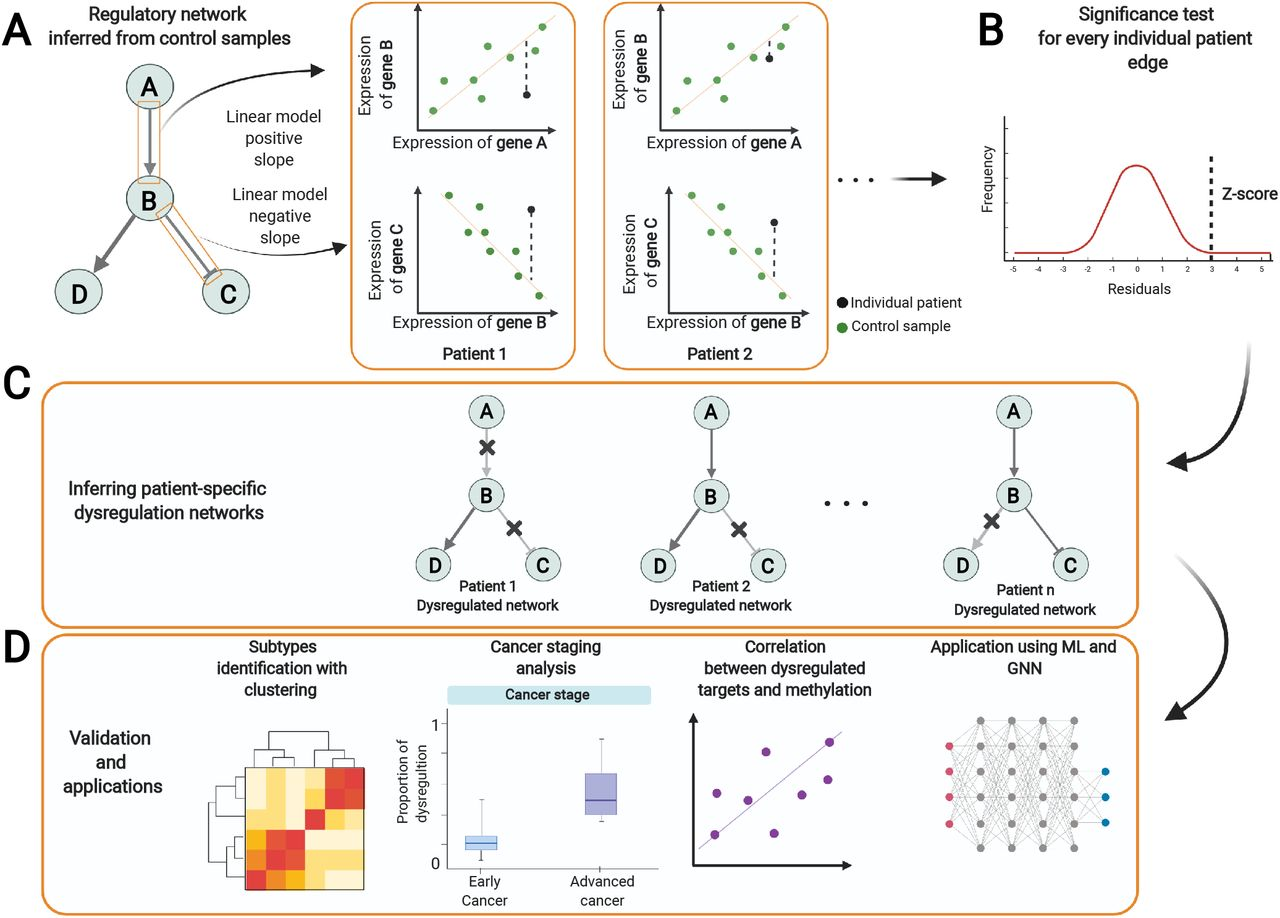
\includegraphics[scale=1.3]{figures/dysregnet.jpg}}
	\caption{A Illustration of the DysRegNet tool and workflow. Showing the fitting of the linear model for each edge, the patient individual significance test, the resulting networks and the subsequent result validation. Figure taken from \cite{dysregnet} without modifications under the Creative Commons CC-BY license.}
	\label{dysregnet}
\end{center}
\end{figure}

DysRegNet does this by fitting a linear model for each edge given by the input GRN using all control samples (Fig. \ref{dysregnet}). The model parameters are estimated in advance using Ordinary Least Squares. Then each patient sample is tested one after the other and the observed value is compared with the expected value from the linear model, which is comparable with an outlier detection task in regression analysis. A test sample specific z-score is calculated using a standardized residual. After analyzing all patients the z-scores are transformed into p-values and corrected for multiple testing. It is important to mention that dysregnet can also account for covariates, which gives the tool an advantage over comparable tools that do not have this feature integrated.

\subsection{CpG-mapping and Beta Values}
\label{beta values}
To use the GRN as input to DysRegNet an expression value for each node is needed. So far, the GRNs only contain expression values for gene nodes. To obtain expression values for the REMs as well, the beta values of all CpGs lying within the REM coordinates  by taking the CPG coordinates from Illumina Methylation450K\cite{methylation450}. 

Since the coordinates of the CpGs are based on GRCh37 and all EpiRegio coordinates are based on GRCh38, the CpG coordinates were mapped to GRCh38 using UCSC LiftOver with default settings\cite{liftover}. LiftOver takes a bed file containing the input coordinates from the selected assembly and convertes them to the coordinates of the desired output assembly. Coordinates that can't be converted result in a list of mismatches, the successfully converted coordinates are printed to a file. After manually filtering 71 mismatches from LiftOver and REMs to which no CpG site could be assigned, all remaining REMs have their assigned CpGs by mapping the CpG site coordinates to the REM coordinate ranges.

The beta values of the CpGs from the data being analyzed were converted to m-values, as these show significantly better performance in identifying differentially methylated CpG sites\cite{mvalues} by the following equation:
\begin{equation}
	m-value = \log_{2}{(\frac{beta}{1-beta})}
\end{equation}
To obtain a single expression value for a REM, the mean was calculated over all m-values of the CpGs contained in a REM.

This provides all input data, the GRN, expression values for all nodes, and the remaining data of respective data set for DysRegNet.

\subsection{LOLA}
LOLA is an R package tool integrated in Bioconductor for enrichment analysis for genomic regions\cite{LOLA}. The analysis is based on testing for overlaps of genomic regions of interest and a database of regions from previous studies.
Three components are needed for the analysis: (I) The query set - several or a list of genomic regions to be tested for enrichment; (II) A region universe - the background set of genomic regions contained in all query subsets; (III) The genomic region reference database to be tested for overlap with the query set. LOLA contains several core databases for the GRCh38 genome, among others and (I) and (II) can be read in as BED files.
\begin{figure}[!ht]
\begin{center}
	\fbox{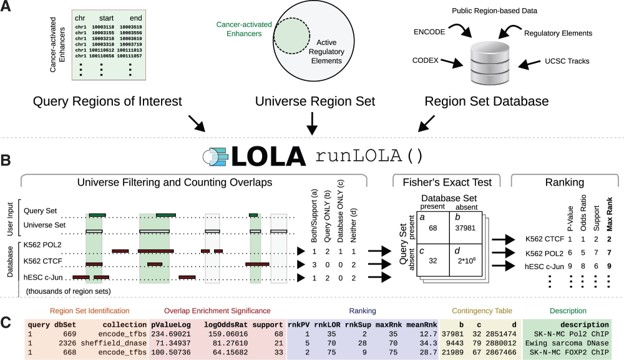
\includegraphics[scale=0.7]{figures/LOLA.jpg}}
	\caption{A Illustration of the LOLA enrichment workflow. Figure taken from \cite{LOLA} without modifications under the Creative Commons CC-BY license.}
	\label{lola}
\end{center}
\end{figure}
LOLA identifies all regions from the query set that overlap with each region set in the reference database, which is performed against the user specified region universe (Fig. \ref{lola}). A single common base pair is sufficient for both regions to be considered overlapping, but can be adjusted by the user. Finally, LOLA uses Fisher's exact test with false discovery rate correction to evaluate the significance of the overlap. The resulting rank score is the worst (max) rank of P-value, log-odds ratio and number of overlapping regions. The resulting enriched regions are returned as a \texttt{data.table} object. This provides a powerful interface for sorting, exploring, visualising and further processing the results.



\section{Network Generation and Data Preparation}
\subsection{Graph-files}
\label{graphfiles}
For the creation of the graph files, all 10 files of the EpiRegioDB were viewed and all samples from the \texttt{sampleInfo\_Roadmap\_1.csv} and \texttt{sampleInfo\_Blueprint\_1.csv} project files were assigned to their cell types with help of the \texttt{CellTypeInfo.csv} file. The samples from both projects were matched with those of the \texttt{REMActivity\_1.csv} file. This resulted in 165 samples in 46 cell types which are stored in the \texttt{sampleToCelltype.csv} file. 

For each cell type, a directed graph file was created containing the edge, the REM and the gene as source and target node from the \texttt{REMAnnotationModelScore\_1.csv} file. As an edge attribute the cell type specific edge weights contained in the cell type were stored as an internal \texttt{edge\_property} from graph-tool under the sample name. As edge weight the value of the standDnase1Log2 column from the \texttt{REMActivity\_1.csv} file was used. REMs associated with a CREM from the \texttt{clusterREMs\_1.csv} file were merged into one CREM node. CREMs have a single edge to the corresponding gene for each contained REM. 
In addition, the all cell type graph file with the identical edges, genes and REMs as nodes was created using the \texttt{REMAnnotationModelScore\_1.csv} file. As edge weight the value of the normModelScore column from the same file was used, which contains the model score across all cell types.
As REM and gene internal \texttt{vertex\_property} node attributes, type, name, chromosome, start, end and for the cell type specific graph files the gene expression for gene nodes for the respective sample were added from \texttt{GeneExpressionBlueprint\_1.csv} and \texttt{GeneExpressionBlueprint\_1.csv}.
As additional edge attributes the rem name of the edge, for the all cell type graph file the p-value and for the cell type specific graph files the cell type and cell type ID were added. 

As already mentioned, depending on whether it is a cell type specific or the all cell type graph, the edge and node attributes differ. To show the attributes values an example the graph for \texttt{CTID\_0000006}, cd14-positive monocyte and the all cell type graph is taken. 
\paragraph{Node attributes:} 
\begin{itemize}
\item name: name of the gene/REM
\item type: node type, either gene oder rem
\item chr: chromosome on which the gene/REM in located
\item start: start coordinate of gene/REM
\item end: end coordinate of gene/REM
\end{itemize}
Only for gene nodes:
\begin{itemize}
\item B\_C0010KB1: expression value in sample B\_C0010KB1
\item B\_C0011IB1: expression value in sample B\_C0011IB1
\item B\_C001UYB4: expression value in sample B\_C001UYB4
\end{itemize}
The all cell type graph contains these node attributes except for the expression values. The reason for this is that this graph contains model score values for all cell types and therefore has no expression value for all cell types at once. 
The difference with the CTID\_0000006 graph concerning the edge attributes is that it has a separate edge attribute for each sample with its name. 
\paragraph{Edge attributes:} 
\begin{itemize}
\item rem: REM name the edge is assigned to, only important if REM is part of a CREM
\item celltype: CTID\_0000006
\item celltypeID: cd14-positive monocyte
\item B\_C0010KB1: standDnase1Log2 value for edge in sample B\_C0010KB1
\item B\_C0011IB1: standDnase1Log2 value for edge in sample B\_C0011IB1
\item B\_C001UYB4: standDnase1Log2 value for edge in sample B\_C001UYB4
\end{itemize}
In the all cell type graph, the same attributes are present except for the standDnase1Log2 values, these are replaced by the following:
\begin{itemize}
\item score: model score over all cell types
\item p-value: p-value for the model score
\end{itemize}
This produces 47 graph files in total with identical nodes and edges, each representing a cell type specific or a GRN for all cell types.



\chapter{Results and Discussion}
In this work, the described methods and a variety of analyses were performed with the aim of finding patient-specific dysregulations in GRNs. For this purpose, 47 GRNs were created, which can be visualized and investigated in an app adapted for this purpose. In the use case, a cancer data set was analyzed for dysregulated REMs using DysRegNet\cite{dysregnet} and these were analyzed for their enriched TFBs using LOLA\cite{LOLA}. 
\section{Network}
The resulting 47 GRNs serve as the basis for all analyses and visualizations. These networks contain several million nodes and edges. In detail every graph consists of:

\renewcommand{\arraystretch}{2}
\begin{table}[!ht]
\centering
\begin{tabular}{|c|c|}
\hline
Number of nodes		& 1.541.001		\\
Number of edges		& 2.404.861		\\
Number of genes		& 35.379        \\
Number of REMs		& 1.140.336		\\
Number of CREMs		& 365.286      	\\
\hline
\end{tabular}
\caption{Element numbers contained in the network graph.}
\label{numbers}
\end{table}
\renewcommand{\arraystretch}{1}
The basic structure of the graphs is composed of small clusters consisting of one gene, which has a large number of incoming edges from REMs and CREMs (Fig. \ref{network}). Genes have exclusively named incoming edges and no edges to other genes. REMs have exclusively a single outgoing edge to their assigned gene and no edge to other REMs. Only CREMs have multiple outgoing edges representing the edges of the contained REMs. CREMs can therefore also have edges to several different genes or several edges to the same gene, each representing a single REM edge. Thus, the mentioned small clusters are connected, if then only by edges from CREMs. Since not every gene has an edge to a CREM and only through it can the individual gene clusters be connected, the network is a disjoint network.
 
Figure \ref{network_webapp}, a section of the webapp visualization, illustrates the individual cases all at once. \texttt{ENSG00000142627} in the upper right corner shows the case where a gene is connected only to REMs and not CREMs, creating an isolated clique with no connection to the rest of the network because REMs can exclusively have a single edge to a gene. The large cluster in the lower left center of the figure with \texttt{ENSG00000236908} and \texttt{ENSG00000275850} shows how two genes are connected via \texttt{CREM0068412}. Here, \texttt{ENSG00000236908} has only one incoming edge through the mentioned CREM and \texttt{ENSG00000275850} forms a cluster with several neighboring REMs and CREMs, while it is also connected to other genes via the latter, but these are not shown here. Also, one can see the case where a CREM has multiple edges to the same gene, each representing a separate REM edge.
\begin{figure}[!ht]
\begin{center}
	\fbox{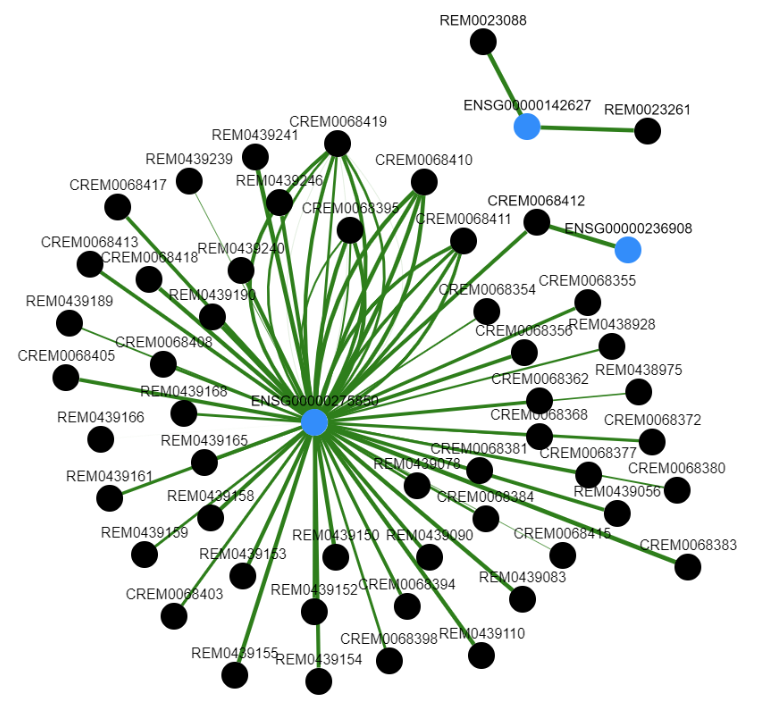
\includegraphics[scale=0.597]{figures/network_webapp1.png}}
	\caption{Visualization of three genes and their connected REMs and CREMs in the Webapp to show the clusters and disjoint structure of the network. Three genes can be seen as light blue nodes, REMs and CREMs are shown as black nodes and are all connected by their edges with edge weight not shown. Source: own work.}
	\label{network_webapp}
\end{center}
\end{figure}

Looking at the topology, the graph consists of 2.188 individual components, which are shielded from each other and cannot be reached by each other. The sizes of the components range from 2 to the largest component with 16.500 contained nodes and form a total of 1.055 different sizes. Smaller components with up to 1.000 contained nodes occur significantly more often than extremely large ones. The most frequent components are those with 55 nodes, of which a total of 134 can be found in the entire network, and the least frequent components with 10.000 nodes or more are usually represented only once. That illustrates that the network consists of many individual components, which differ strongly by their size and frequency.


The average degree over all nodes within the graph is 3.12, but it differs enormously if you look at the node-types. The average degree for gene nodes is 67.97 (Fig. \ref{gene_degree}) and for REM and CREM nodes only 1.60. This value is small for REM and CREM nodes, since REMs always have only one edge to a certain gene and thus drive the average value down. Looking at the average degree for CREMs only, it is almost three times higher at 3.46 (Fig. \ref{crem_degree}). These numbers again describe the network structure with clusters of genes with many incoming edges from regulatory elements. The value of the maximum degree does not differ that much and is 108 for gene nodes and 122 for CREMs, for REMs the value is 1.0 since they are connected through only one edge. However, 8.096 genes have a degree of 108, only \texttt{CREM0109128} (Fig. \ref{crem_max_degree}) has a degree of 122, which is enriched for the nuclear respiratory factor 1 gene (NRF1) using LOLA\cite{LOLA}. NRF1 functions as a TF, activating the expression of genes required for mitochondrial DNA transciption and regulating cellular growth\cite{NRF1}. The TF is thus involved in many processes and therefore has a high number of interactions.
The degree distribution of the CREMs (Fig. \ref{crem_degree}) is very one-sided and most of them have degrees of 2 and from fifteen on there are only a few with higher degrees. The distribution of gene degrees (Fig. \ref{gene_degree}), on the other hand, looks very different with two maxima at 54 and 108, showing that a maximum degree of 108 is a common case. 

Results that support these findings can also be seen by looking at the clustering coefficients, which give 0 for both local and global clustering coefficients.  For this purpose the methods \texttt{local\_clustering} and \texttt{global\_clustering integrated} with default settings from graph-tool were used. These minimal coefficients show that all nodes in this network have no edges between their neighboring nodes, and thus only nodes are connected to their immediate neighbors. This confirms the description of the basic network structure as described earlier.



\section{Web Application}
To be able to interact with the created graph files, a user friendly web application (app) was designed. The app provides visualization, interaction and filtering of the networks and their properties for user specific usage. It was created as described in \ref{dash} using dash and dash-cytoscape.

\subsection{Structure}
The basic structure of the app is divided into three parts, which are arranged vertically next to each other. In the left column, the data can be selected for display and there is the option for a file upload. In the middle column is the display area of the elements selected in the left column. In the right column you can filter the elements to be visualized and display information about selected nodes. 

\begin{figure}[!ht]
\begin{center}
	\fbox{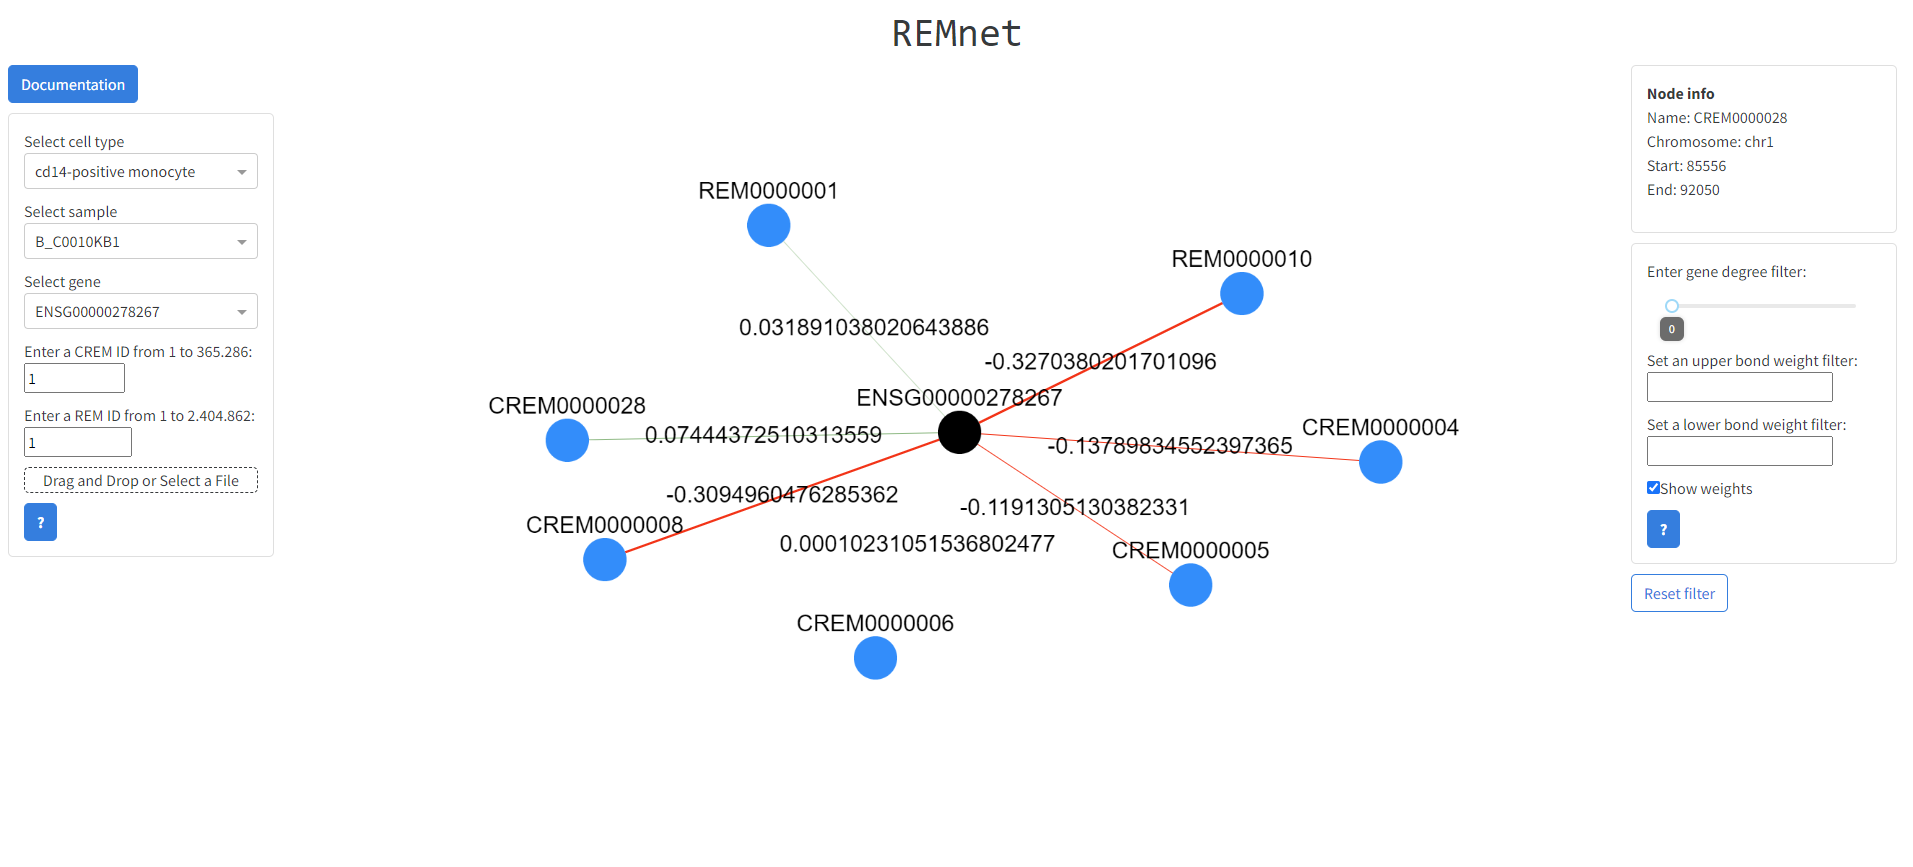
\includegraphics[scale=0.389]{figures/webapp.png}}
	\caption{App view on start with the selection options on the left, the visualization in the middle and the filtering on the right. Source: own work.}
	\label{webapp}
\end{center}
\end{figure}

\subsection{Selection}
The left column is the selection column. It has two help buttons for the user, which can be opened and closed like all help button by simple clicks. The \texttt{Documentation} button gives an overview of which actions can be performed in which parts of the app.
The \texttt{?} help button gives instructions to the user on how to use the selection and upload options.

Below that is the window for all display choices. In the first \texttt{Select cell type} drop-down menu, all cell types contained in Roadmap\cite{roadmap} and Blueprint\cite{blueprint} can be selected. Selecting one of the cell types will reload the respective graph file as described in \ref{graphtool}. This results in a additional short loading time, but allows to speed up the subsequent work in the graph file. For the loading time a spinning loading circle is displayed in the upper center of the page. Below that, it is possible to choose from all the samples available for this cell type in the \texttt{Select sample} drop-down. If the all cell type graph is selected, the model score and the p-value are selectable instead of the sample names as explained in \ref{graphfiles}. In the next three input fields, genes, REMs or CREMs can be selected. Only one of the three can be shown in the visualization, the last selection is always shown. In the gene \texttt{Select gene} drop-down menu, genes can be selected by their ensemble ID. For the selection of REMs and CREMs, the desired ID must be entered. All drop-down menus can be searched for the desired selections. 

In addition to the above options, the user can upload a CSV file with individualized nodes and edges. This function is useful if only selected or several disconnected elements are to be displayed. The file must be in the format \texttt{'REM,GENE'} as header with two columns where each row describes an edge between the respective REM and Gen. Other file formats and formattings are not accepted.

\subsection{Visualisation}
In the app center, individual genes, REMs, CREMs and their neighboring nodes and edges or a user-defined input of nodes by the file upload can be displayed.

When a gene, REM or CREM is selected, it is displayed as seed node in black. All neighboring nodes are displayed in light blue and the edges leading to them. Above each node the corresponding name is displayed. Depending on the previously selected sample, the adjusted edge weights are shown on the edges. For a simplified illustration, the edges are colored green for positive edge weights and red for negative edge weights. In addition, the edge width adapts to the weights and becomes wider the further away the value is from 0. If the file upload function is used, all edges specified in the file are displayed. Genes are always displayed as black nodes and REMs and CREMs as light blue nodes (Fig. \ref{network_webapp}). 

These display options are available, since the display of the entire GRN is not useful for several reasons. On the one hand, it would be extremely inefficient, creating long loading times and thus a poor user experience. On the other hand, the display of the entire GRN would be confusing and the user would have difficulties to orientate himself, as in Fig. \ref{complete_network}. 

\subsection{Filtering}
The right column of the app contains information about nodes and filtering options for the GRN. 
In the upper bin, information about nodes for which more details are requested can be displayed. The information appears by simply clicking on a node. The name of the node, on which chromosome it is located and the start and end position in the genome are given. The display is available for genes as well as REMs and CREMs. 

The box below contains the filter options for the network visualization. With the help of the first \texttt{Enter gene degree filter} slider the gene degree can be filtered. By moving the slider, genes with a higher gene degree than the filter value are filtered. This affects the \texttt{Select gene} dropdown menu where the selectable genes are adjusted according to the filter. In the \texttt{Upper bond weight filter} and \texttt{Lower bond weight filter} input fields the edge weights can be filtered. In the former, edge weights smaller than the filter are filtered and larger ones are left out. With the latter it is the opposite, edge weights larger than the filter are filtered and smaller ones are left out. Thus, the edge weights can be narrowed down from both sides. The filters are transferred to the visualization after selection and all edges excluded by the filters and nodes connected only by the excluded edge are removed. Using the \texttt{Show weights} select box, the edge weights can be shown or hidden. The \texttt{?} help button gives instructions to the user on how to use filters correctly. The \texttt{Reset filter} button resets all selected filters to their default values. 

All these functions and filters together form the app, which allows the user to view and filter desired parts of the GRN.  

\section{Use case}
The GRN can be applied in combination with DysRegNet and LOLA to identify and investigate patient-specific dysregulations in a disease data set. A corresponding use case is described below for publicly available breast cancer data (BRCA).

\subsection{Breast Cancer}
\label{breast cancer}
With 2.3 million new cases of BRCA, it is the most common type of cancer in women\cite{brca_general}. Breast cancer also affects men, who account for less than 1\% of breast cancer cases. The risk of developing breast cancer also depends on several factors, among which the mutations in the tumour suppressor genes BRCA1/BRCA2 and older age contribute negatively. Numbers of cases and the death rate increased between 1990 and 2016. Death rates have doubled in 60 of 102 countries such as Saudi Arabia and Paraguay, and even tripled in ten countries such as Iran and Algeria. The number of cases also more than doubled in 43 of 102 countries, such as Afghanistan and Brazil\cite{brca_history}. Survival depends on both stage and molecular subtype. Looking at the histology, BRCA can be divided into subtypes Luminal A, Luminal B, HER2 enriched, Basal-like and Normal Breast-like. The subdivision is based on different gene expression levels such as those of estrogen receptors (ER), progesterone receptors (PR) or human epidermal growth factor receptor 2 (HER2).
\begin{figure}[!ht]
\begin{center}
	\fbox{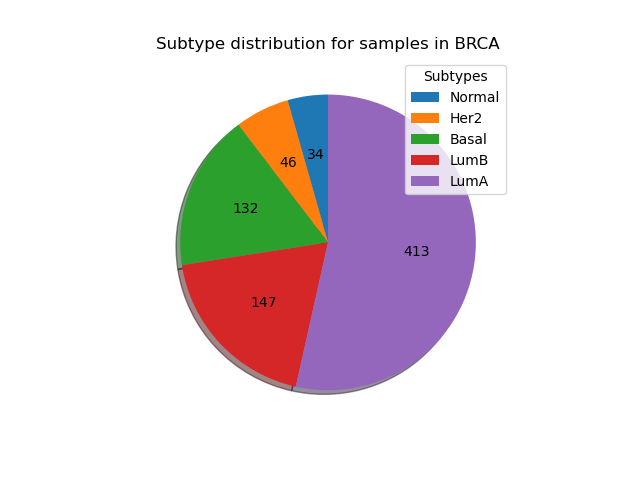
\includegraphics[scale=0.5]{figures/subtype_distribution.png}}
	\caption{Distribution of subtypes numbers in samples of the DysRegNet result from TCGA\cite{tcga} BRCA data set. Source: own work.}
	\label{subtypes}
\end{center}
\end{figure}
Luminal breast cancers account for almost 70\% of all breast cancers in the western population and are characterized by the presence of ER. Luminal A and Luminal B breast cancers are differentiated by the absence of PR and/or the presence of HER2 in Luminal B tumours. The HER2-enriched subtype, which is characterized by a high expression of HER2 and the absence of ER and PR, accounts for 10-15\% of breast cancer cases. Basal-like, often used interchangeably with triple-negative breast cancer, is characterized by the absence of both ER and PR as well as HER2\cite{brca_general}. This subtype accounts for about 20\% of breast cancers. The Normal Breast-Like subtype accounts for between 5-10\% of breast cancer cases, but is poorly characterized as its gene expression levels are intermediate between Luminal and Basal-like subtypes\cite{brca_normal_like}.

The Xena platform\cite{xena} contains the \texttt{GDC TCGA Breast Cancer (BRCA)} data set with meta data, expression data and methylation data for breast cancer patients from The Cancer Genome Atlas (TCGA)\cite{tcga}. The meta data contains 1.284 samples with 140 identifiers each, distributed across both sexes, several ages, with a control group and others. The expression data contain values for 1.217 samples over 60.484 genes. The expression values are FPKM (Fragments Per Kilobase Million) and log2(x+1) transformed values. The methylation data consist of 890 samples and 485.578 CpGs containing the respective beta values for Methylation450K\cite{methylation450}. 

\subsection{DysRegNet}
Given a disease dataset, there is interest in finding dysregulations in REMs that differ between case and control samples, as these can be used to infer the changes in affected patients. With the help of DysRegNet, patient-specific dysregulations of gene expression profiles can be inferred.

\begin{figure}[!ht]
\begin{center}
	\fbox{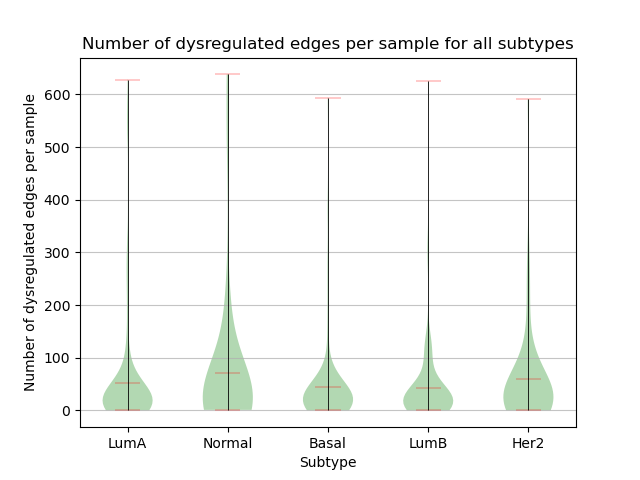
\includegraphics[scale=0.7]{figures/edges_per_sample_violin.png}}
	\caption{Number of dysregulated edges per sample on the x-axis in the DysRegNet result. Grouped by BRCA subtypes on the y-axis. Source: own work.}
	\label{edges_per_sample}
\end{center}
\end{figure} 
For the DysRegNet inputs, the data was adapted accordingly. The GRN was extracted from the all cell type graph file in the form \texttt{REM - GENE} for all edges contained. In the meta table, the control samples were encoded with 0 and the case samples with 1. Missing values for in the \texttt{days\_to\_birth.demographic} column were completed with the mean column value. With the help of the methylation data, the CpGs were matched to their respective REMs as described in \ref{beta values}, the beta values were converted to m-values and the mean value of all contained CpGs was assigned to each REM as expression value. 
The REMs and their newly generated expression values were added to the expression table. Since the meta data, the expression table and the methylation data do not contain the same samples, they were filtered to the largest intersection for all three tables. In the GRN, the REMs and genes were adjusted according to those contained in the expression table, since not all REMs could be assigned CpGs and thus expression values.
\begin{figure}[!ht]
\begin{center}
	\fbox{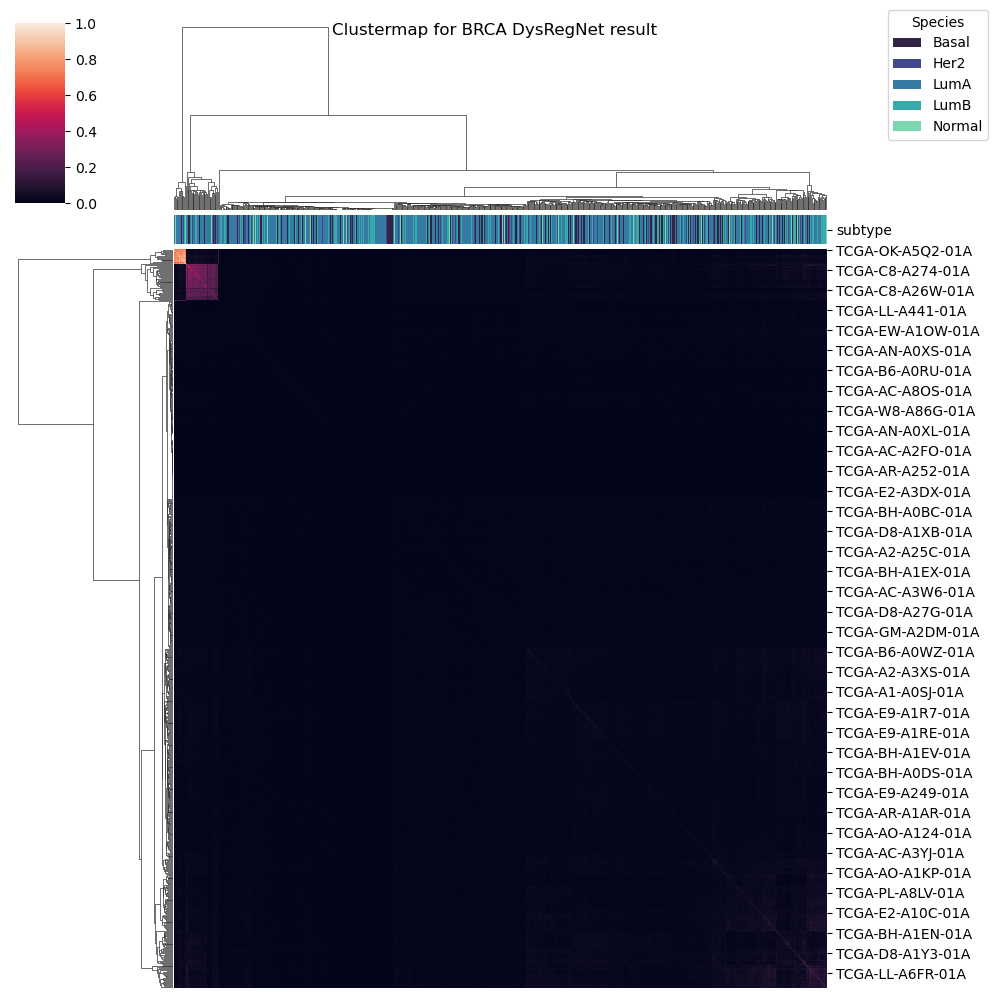
\includegraphics[scale=0.6]{figures/BRCA_clustmap.png}}
	\caption{Clustering Heatmap of the number of equal dysregulated edges for each pair of samples plotted on both axes. The x-axis shows the respective subtypes of the samples and lighter values in the matrix indicate a higher number of equal dysregulated edges per sample pair. Source: own work.}
	\label{brca_clustmap}
\end{center}
\end{figure} 
This results in 861 samples in the meta table as well as the Expression table. The input GRN and expression table values contain entries for 75,543 REMs and 34,934 genes.
To run DysRegNet, the default input values as in the example of the DysRegNet paper\cite{dysregnet} were taken. Thus the inputs are: (I) expression, meta and methylation tables described above; (II) covariates race, gender and days to birth; (III) R2 threshold = 0.2 and normaltest = True; (IV) sample type as condition column.
The result was a table with 778 case samples and 169,498 predicted dysregulated edges connecting REM and gene. If only the edges that have a z-score unequal 0 in one of the samples are considered and are thus predicted dysregulated, 1.890 edges remain. Only named dysregulated edges are used for further analysis. 

To get a better and more detailed understanding of the resulting dysregulated edges and to see if they can be subdivided by their patterns into BRCA subtypes they were further analyzed. The edges were clustered to obtain subtype specific groups of samples and thus of the dysregulated edges. 
To achieve this, the samples were assigned their subtypes. For the assignment, the table of PanCancerAtlas subtypes from TCGAbiolinks\cite{tcgabiolinks} was used. It was filtered according to the cancer type BRCA and the samples for which a subtype is given. This resulted in a table of 772 samples with their associated subtypes. In the BCRA subtype distribution (Fig. \ref{subtypes}), it is noticeable that the luminal subtypes make up almost two-thirds of all samples, as they account for the largest proportion of breast cancer cases, described in \ref{breast cancer}. The HER2 and basal subtypes represent the smallest groups. 
Looking at the number of dysregulated edges per sample (Fig. \ref{edges_per_sample}), it becomes apparent that the distributions for each subtype are similar. The distributions differ minimally in their maximum values around 600 and their mean values do not diverge much. This provides a good basis for differentiating the subtypes according to their dysregulated edges, as they are comparable. In contrast, the subtype distributions for the number of dysregulated samples per edge differ significantly (Fig. \ref{samples_per_edge}). They are proportionally similar to the sizes of the subtypes in figure \ref{subtypes}. This is due to the fact that samples from the larger subtypes are more likely to be dysregulated in more edges.

For the clustering of the edges, all edges were compared with each other in pairs. For each pair, the number of edges that are dysregulated in both samples, i.e. have a z-score unequal 0, was determined. This results in a symmetrical matrix with all samples on both the x- and y-axis, with the number of equal dysregulated edges in each cell. The matrix was normalized in order to obtain values between 0 and 1. Clustering this table using a clustering heatmap and displaying the corresponding subtypes of samples yields the result in figure \ref{brca_clustmap}. 
The samples do not cluster into their subtypes as expected. Two clusters can be seen in the upper left, however, these are divided across all subtypes and therefore are not subtype-specific. Apart from that, no other clusters are visible.

\subsection{LOLA enrichment}
\begin{figure}[!ht]
\begin{center}
	\fbox{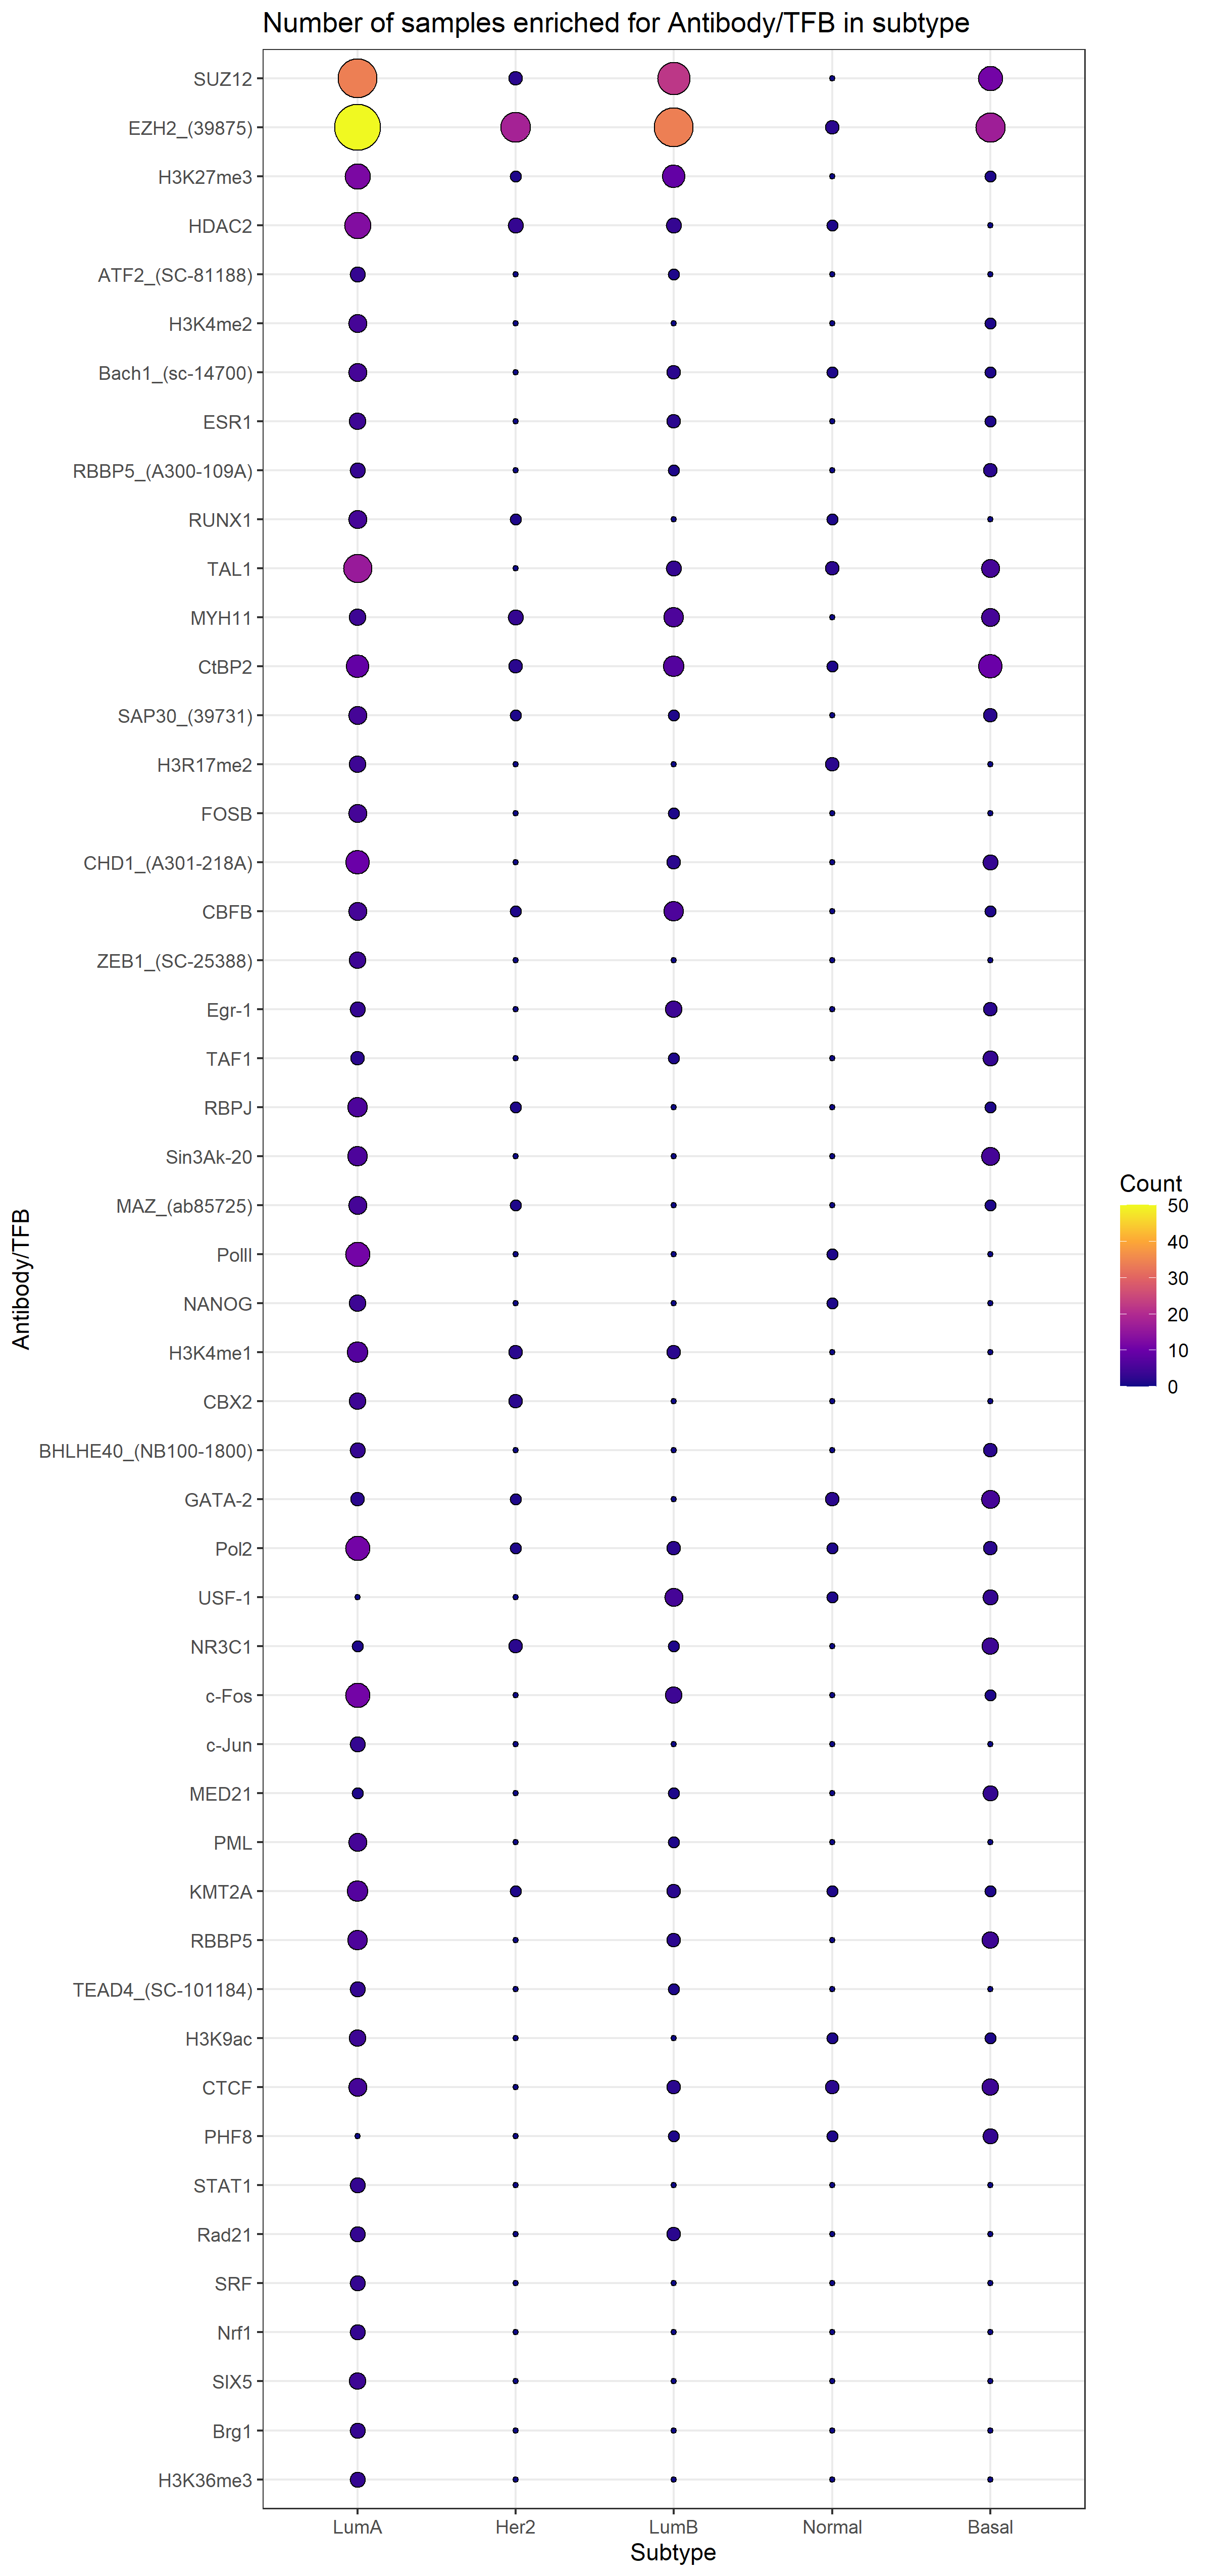
\includegraphics[scale=0.45]{figures/lola_matrix_filt_max.png}}
	\caption{Illustration for the number of samples in which the TFBs is enriched on the x-axis, shown for each subtype on the y-axis. Source: own work.}
	\label{lola_result}
\end{center}
\end{figure} 
The DysRegNet results provide dysregulated edges between REM and gene per case sample. However, only genomic coordinates are given for the REMs. Therefore, it is interesting to investigate which TFBs represent the dysregulated REMs. For this purpose, the LOLA enrichment tool was used, which provides an enrichment analysis for genomic regions. 
From the DysRegNet results table, a \texttt{.bed file} was created for each sample containing the coordinates of the REMs in the dysregulated edges. Samples without dysregulated edges were filtered out, leaving 746 samples and \texttt{.bed files}. These were taken as query sets and the hg38 genome from the LOLA core data base as the data base for input. All edges from the DysRegNet result table that were dysregulated in at least one sample formed the region universe for input. The LOLA results provide the enriched TFBs for the REMs from each sample file. For each TFBs, the results of the statistical test are given by p-value, log-odds ratio, number of overlaps and ranks. The meanRank and maxRank rank the results using a combination of named values and often provide the most interpretable results\cite{LOLA}. 
The results for each sample were ordered by their ascending maxRank and TFBs with the smallest maxRank were taken. By calculating the number of taken enriched TFBs of all samples per BRCA subtype, a table with subtypes on the x-axis and all uniquely enriched TFBs on the y-axis was generated. The table was filtered for all TFBs that occur at least twice in a subtype. This leaves 50 TFBs and their number of occurrences in the five BRCA subtypes (Fig. \ref{lola_result}).

Looking at Figure \ref{lola_result}, EZH2 and SUZ12 are significantly more abundant than others in all subtypes except Normal. This shows us that REMs of EZH2 and SUZ12 are dysregulated in many of the case samples compared to the control samples in almost all BRCA subtypes. EZH2 and SUZ12 are both subunits of the Polycomb group protein PRC, whose target gene expressions have been shown to be downregulated in basal-like breast cancers. PRC possesses histone methltranferase activity and primarily methylates H3K26me3, which in addition as seen is also dysregulated in increased numbers\cite{PRC2}. EZH2 is involved in tumorigenesis including cell differentiation and stem cell maintentance. It is reported to be elevated in aggressive metastatic tumors and is an independent predictor of survival\cite{EZH2}. 
CtBP2, a member of the C-terminal binding protein group (CtBP) that regulates several different cellular functions in vertebrates, shows an increased number of dysregulations as well\cite{CtBP2_general}. Among others, it plays a central role in the transcriptional regulation of BRCA1 and the overexpression of CtBP2 has been linked to breast cancer\cite{CtBP2}. 
To view the observed dysregulated REMs in the context of the GRN, they can be visualized using the app. Through the display, the regulatory connections to genes become apparent. The relationships between REMs and genes can be further analyzed on a cell type specific level. 




\chapter{Conclusion and Outlook}
This work shows how the patient specific dysregulation analysis can be performed based on a GRN for a TCGA BRCA dataset\cite{tcga}. For this purpose, several GRNs were generated from epigenetic data from EpiRegioDB on REMs and their regulatory connections to genes. To analyze a GRN for patient-specific dysregulations, the DysRegNet tool was used. Since the REMs do not have expression data, these were therefore regenerated using the beta values from the TCGA BRCA dataset. Beta values were converted to m-values and the average value of these over all CpGs contained in a REM was assigned. The resulting dysregulated edges and their contained REMs were analyzed using LOLA and other methods. Results from LOLA show that enriched TFBs from dysregulated REMs, such as for proteins EZH2, SUZ12, H3K26me3 and CtBP2, found in increased numbers disease tissue are already associated with altered regulations in BRCA. The results found can be visualized in the app that allows REMs, genes and their regulatory relationships to be displayed interactively, filtered and cell and sample specific.

The performed analyses and work can be well extended by additional ones. Extensions could be features to perform more detailed research on found dysregulated REMs and their genes. In the app, the ability to display individual components of the GRN would help the user to analyze larger parts of the network than individual REMs or genes. The same advantage would be given by displaying multiple REMs and genes.
The workflow of analyses allows the used breast cancer dataset and the GRN to be extended by others. 
Dysregulation analysis with DysRegNet can be performed with cell type specific GRNs to determine results on cell type level. Data sets containing the required data for other epigenetic diseases can be  integrated and analysed using the same workflow. This includes other cancer datasets as well as datasets for, for example, hepatitis C virus or diabetes mellitus.

The findings show that using the GRN, DysRegNet and LOLA, a patient-specific network-based dysregulation analysis provides further usable results for dysregulated REMs, which can be visualized using the app. This provides the basis for further investigation of newly found dysregulated REMs to discover new insights in cancer research.




\medskip
\clearpage
\bibliographystyle{unsrt}
\addcontentsline{toc}{chapter}{References}
\bibliography{references}

\pagebreak
\appendix
\chapter{Appendix}
\begin{figure}[!ht]
\begin{center}
	\fbox{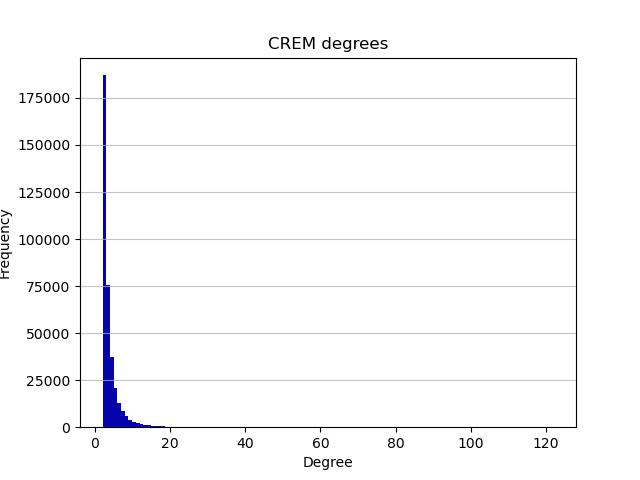
\includegraphics[scale=0.7]{figures/crem_degree.jpg}}
	\caption{Distribution of CREM degrees in GRN. Source: own work.}
	\label{crem_degree}
\end{center}
\end{figure}

\begin{figure}[!ht]
\begin{center}
	\fbox{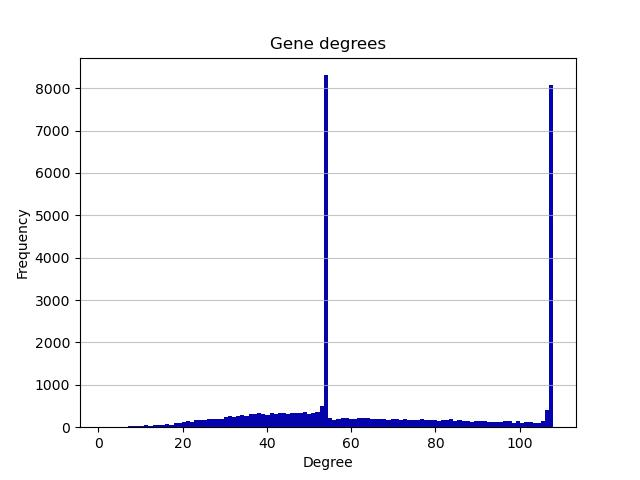
\includegraphics[scale=0.7]{figures/gene_degree.jpg}}
	\caption{Distribution of gene degrees in GRN. Source: own work.}
	\label{gene_degree}
\end{center}
\end{figure}

\begin{figure}[!ht]
\begin{center}
	\fbox{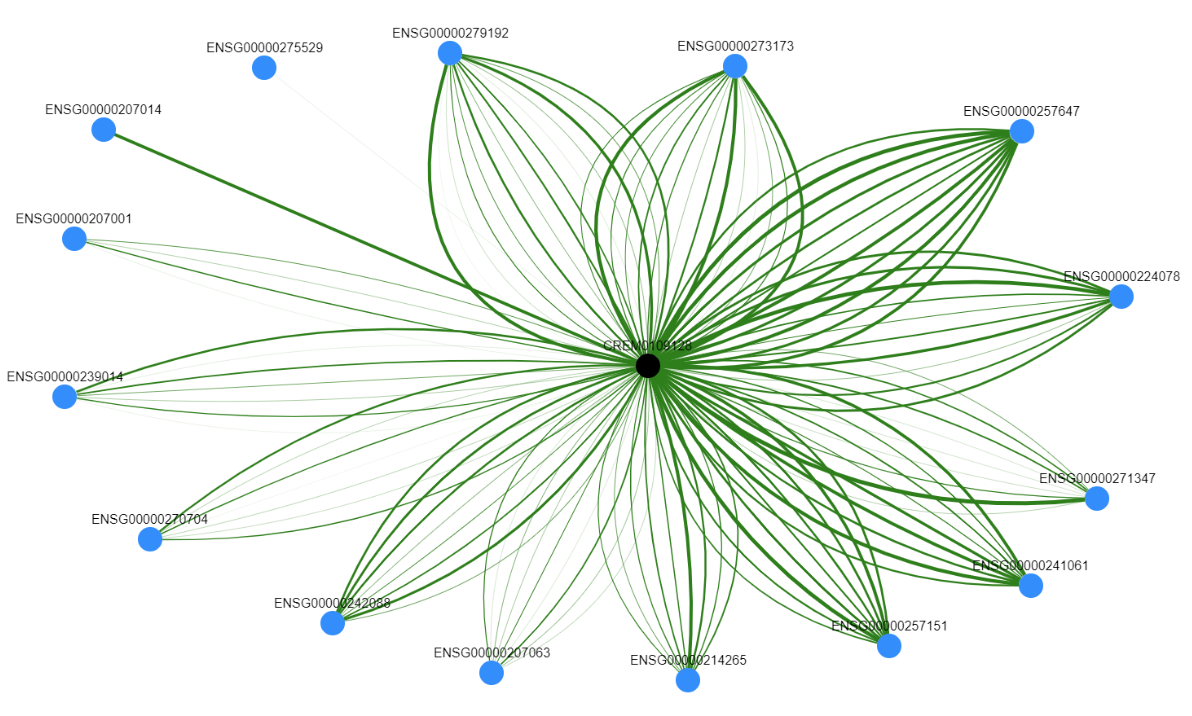
\includegraphics[scale=0.6]{figures/CREM0109128_vis.png}}
	\caption{Visualization of CREM0109128 with maximum degree in the web app. Source: own work.}
	\label{crem_max_degree}
\end{center}
\end{figure}

\begin{figure}[!ht]
\begin{center}
	\fbox{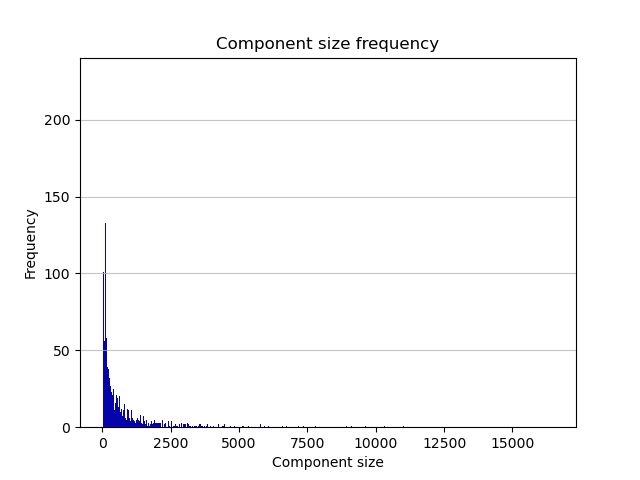
\includegraphics[scale=0.7]{figures/comp_size_freq.png}}
	\caption{Frequency of all component sizes in the network. Source: own work.}
	\label{comp_freq}
\end{center}
\end{figure}

\begin{figure}[!ht]
\begin{center}
	\fbox{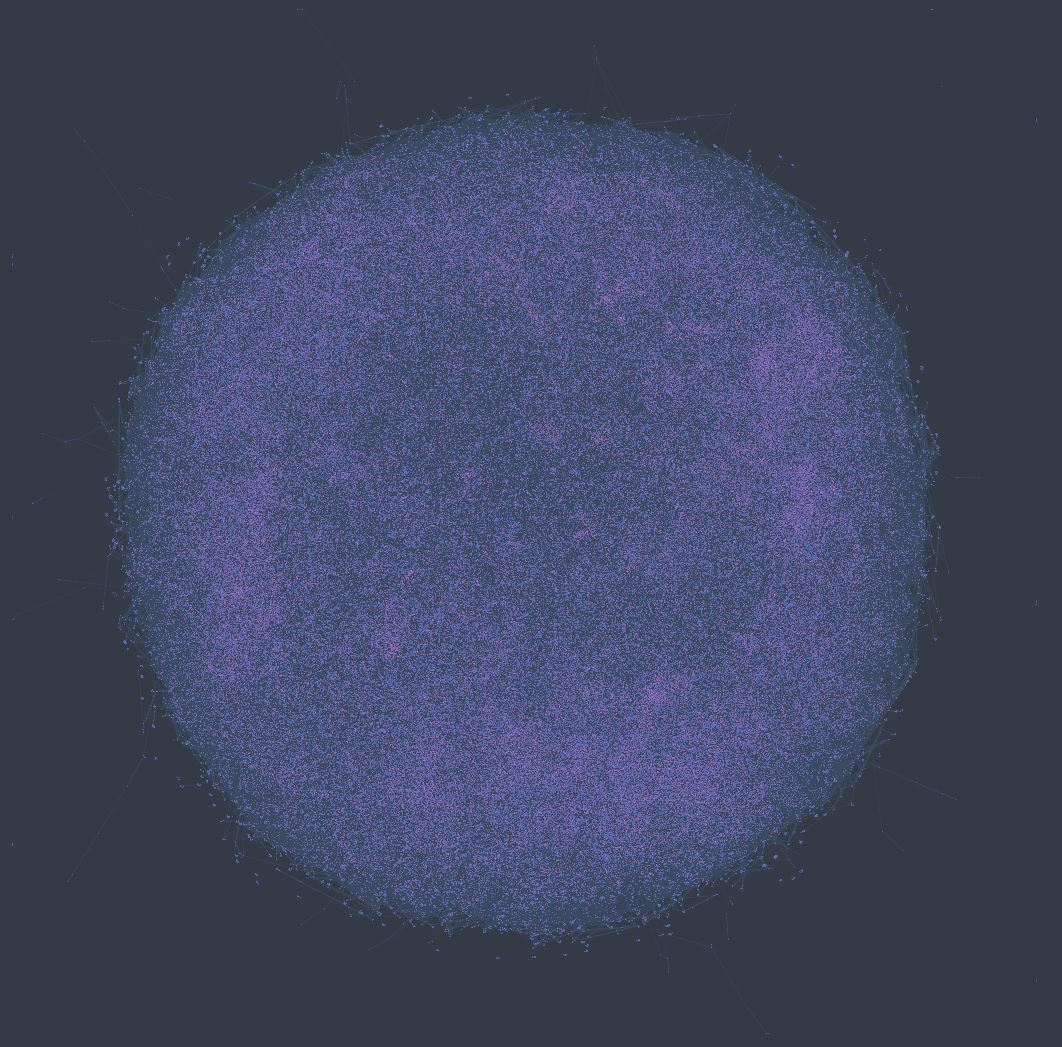
\includegraphics[scale=0.7]{figures/REMnet_rund.jpg}}
	\caption{Visualization of the entire with all nodes and edges. Figure produced with Cosmograph\cite{cosmograph} without modifications under the Creative Commons CC-BY license.}
	\label{complete_network}
\end{center}
\end{figure}

\begin{figure}[!ht]
\begin{center}
	\fbox{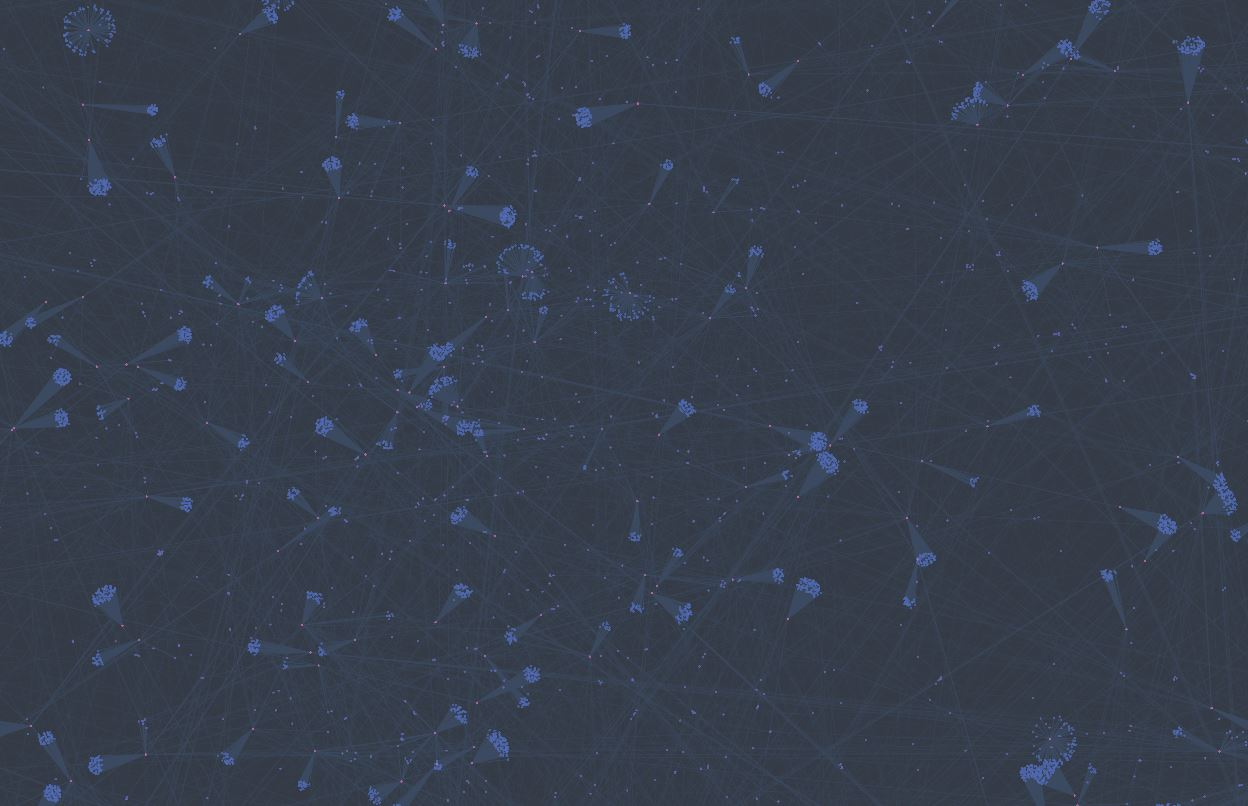
\includegraphics[scale=0.597]{figures/REMnet2.JPG}}
	\caption{Part of the model score network graph showing the clusters with one gene and multiple connected REMs and CREMs. Figure produced with Cosmograph\cite{cosmograph} without modifications under the Creative Commons CC-BY license.}
	\label{network}
\end{center}
\end{figure}

\begin{figure}[!ht]
\begin{center}
	\fbox{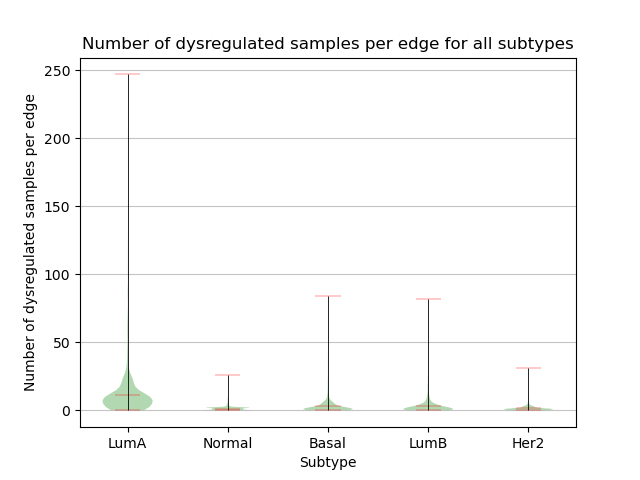
\includegraphics[scale=0.7]{figures/samples_per_edge_violin.png}}
	\caption{Number of dysregulated samples per edge in the DysRegNet result. Grouped by BRCA subtypes. Source: own work.}
	\label{samples_per_edge}
\end{center}
\end{figure}

\end{document}